\section{Introduction}
\label{sec:intro}
     Long short-term memory or LSTM~\cite{hochreiter1997long} is 
a prevalent model which have achieved great results in many 
natural language processing tasks, such as text classification, speech recognition. However, in order to obtain high classification accuracy on deep models, large number of samples have to be labeled manually. This inefficient human labeling process hinders artificial intelligence companies from deploying machine learning applications like training a chat robot or intelligent customer service system. Therefore, how to train a deep model with as few labels as possible has been of great importance to solve.
     
Active learning is a meta-learning framework that aims at
achieving good accuracy with less labeled training data by selecting 
the most informative samples to label, based on criteria
such as variation ratio~\cite{freeman1965elementary}, 
mean standard deviation \cite{kampffmeyer2016semantic}, the 
mutual information between predictions and model 
posterior~\cite{houlsby2011bayesian}.
It has been used in text classification scenarios with 
conventional classifiers, such as 
Exception-Maximization (EM)~\cite{mccallumzy1998employing}, 
Support Vector Machine (SVM)~\cite{tong2001support}, etc.
However, very little work has been done on combining active learning 
with deep neural models. 
     
The reason for the slow development of active deep neural learning
is i) since deep models require more data to converge, at the early
stage of active learning when the samples are small, the intermediate
models thus learned are very unreliable, 
undermining the sampling decisions as well; and ii) 
deep models typically learn and inference more slowerly, and since these 
two steps are repeated executed in active learning, the whole learning
process will be subtantially longer than simple models such as LR and SVM.

%Directly transplanting traditional sampling strategies 
%on deep models often provides disappointing results at the early 
%stage of active learning, since most sampling strategies follows 
%the information given by the classifier, like calculating the 
%Even the state-of-the-art method \cite{zhao2017deep} only do some elaborations on the information provided by the model.
% 

   
To show the challenge of using deep models on small data, 
Table \ref{tab:accuracy} gives the f1-score of SVM and LSTM trained on 
a data set of 10 short text messages and their labels 
taken from a customer service conversations. 
The performance of the LSTM model is generally worse than SVM. 
     \begin{table}[th]
     \small
    \centering
    \setlength{\tabcolsep}{1.5mm}{
    \begin{tabular}{crr}
    \hline
    Classes& SVM & LSTM \\
    \hline
    3&0.04023&0.04018\\
    4&0.2155&0.1943\\
    141&0.0355&0.0059\\
    \hline
    \end{tabular}}
    \caption{accuracy on different classes with training set size 10}
    \label{tab:accuracy}
    \end{table}
     
Moreover, in noisy data sets, boundary cases can reduce the 
margin gained by applying previous sampling strategies. 
\figref{fig:noise} shows some noisy short texts taken from 
the customer service conversations. 
Previous active learning strategies almost exclusively make sampling decision
on the labels ($y$), without considering the data itself ($x$). 
Hence they may select the the very similar samples ``How to follow", 
leading to limited improvement of the model. 
Furthermore, in many-class classification problems. The differences in
labels can be very subtle. For example, in \figref{fig:noise}, 
``How to get a discount" is a question often asked by customers 
before the purchase, while ``How to get a discount on the shipping" 
is a typical bargain question on the shipping charge. Obviously, 
these two very similar messages belong to two difference classes, 
but with little training data, it is extremely difficult for deep models 
to classify it well.

    \begin{figure}[th]
    \begin{center}
    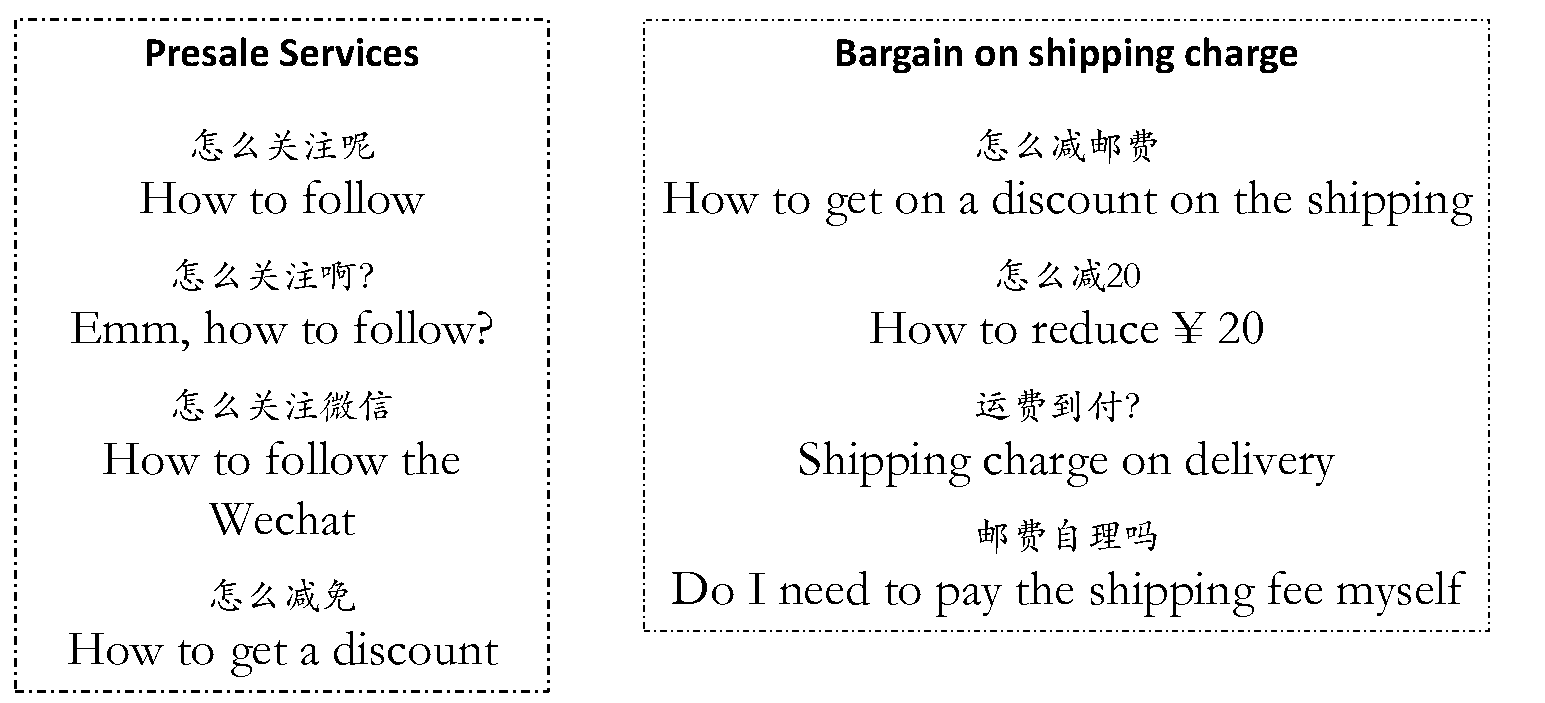
\includegraphics[scale=0.3]{noise.pdf}
    \caption{Noisy data of the same class}
    \label{fig:noise}
    \end{center}
    \end{figure}
     
    
Based on the above observations, we have designed a new paradigm which incorporates both the information provided by the classifier as well as the underlying data itself. In this paper, we propose a hybrid active learning framework tailored for deep models. Our contributions are as follows: 
(1) we design a brand new framework taking advantage of
the features of underlying data as well as the output from the classifier; 
(2) our framework outperforms other strong active learning approaches on 
an E-commerce data set; 
(3) we show that the model is \KZ{less} sensitive to noises in the data set; 
(4) we show that the model can provide comparable results with 
original LSTM trained on whole data set at a relatively early stage
with small amount of data.
